\ifx \globalmark \undefined %% This is default.
	\documentclass[a4paper,12pt]{report}

%%% PACKAGES %%%

\usepackage[french, english] {babel}	% langue principale
\usepackage[ansinew]{inputenc}
\usepackage[T1]{fontenc}		% Police contenant les caractères français
\usepackage{lmodern}			% plus beau
\usepackage[a4paper]{geometry}
	\geometry{hscale=0.75,vscale=0.8,centering}

\usepackage[hidelinks]{hyperref} % pas de couleurs ici
%
\usepackage[natbibapa]{apacite}

%% Maths
\usepackage{amsfonts} % Equations etc
\usepackage{amsmath}
\usepackage{mathtools}
\usepackage{amssymb}

\usepackage{cleveref}

%% Itemizes
\usepackage{enumerate}
\usepackage{enumitem}

%% Dessins & Plots
\usepackage[pdftex]{graphicx} %Images dans le PDF
\usepackage{epstopdf}
\usepackage{color, xcolor}
%% Dates
\usepackage{datetime}
\newdateformat{monthyeardate}{\monthname[\THEMONTH] \THEYEAR}
\usepackage{chessboard}
\usepackage{booktabs,tabularx,multirow}
\usepackage[babel=true,kerning=true]{microtype}
%> Tikz
\usepackage{tikz}
\usepackage{hf-tikz}
\usetikzlibrary{
	calc,
	arrows,
	arrows.meta,
	automata,
	shapes,
	snakes,
	positioning,
	decorations,
	decorations.text,
	fit,
	matrix,
	mindmap
	}
	\tikzstyle{noeud-std}=[draw,fill=black,circle,inner sep=0pt,minimum size=7pt]% 7pt est la taille des cercles noirs
\usepackage{tkz-graph}
\newcommand{\tikzmark}[2]{\tikz[overlay,remember picture,baseline=(#1.base)] \node (#1) {#2};}
\newcommand{\Highlight}[1][submatrix]{%
    \tikz[overlay,remember picture]{
    \node[highlight,fit=(left.north west) (right.south east)] (#1) {};}
    }
\tikzset{%
  highlight/.style={rectangle,rounded corners,fill=ocre!50,draw,
    fill opacity=0.5,thick,inner sep=0pt}
}
\newcommand{\mytikzmark}[2]{\tikz[overlay,remember picture, baseline=(#1.base)] \node (#1) {#2};}


%% Meta
\usepackage{etoolbox}

% Debugging purposes: Catch when a reference is missing
\makeatletter
	\patchcmd{\@setref}{\bfseries ??}{{\color{red}[\texttt{\detokenize{ #3 }}]}}{}{%
	  \GenericWarning{}{Failed to patch \protect\@setref}}
	\patchcmd{\@citex}{\bfseries ?}{{\color{red}[\texttt{\detokenize{ #3 }}]}}{}{%{{\color{red}\texttt{\@citeb}}}{}{%
	  \GenericWarning{}{Failed to patch \protect\@citex}}
\makeatother

%% CUSTOM ENVIRONMENTS
% Packages
\usepackage{framed}
\usepackage{mdframed}
\usepackage[amsmath,thref, framed]{ntheorem}

%% Counters for theorem.
% The current choice is that all environments share a counter within chapters.
% It that regards, it becomes easy to navigate the document.

\newcounter{theo}[chapter]\setcounter{theo}{0}
\renewcommand{\thetheo}{\arabic{chapter}.\arabic{theo}}



% The following is adapted from https://texblog.org/2015/09/30/fancy-boxes-for-theorem-lemma-and-proof-with-mdframed/
% \newenvironment{name}[args]{begin_def}{end_def}
\newenvironment{generic_theo}[2][] % 2 arguments, and one is optional. The first argument will say if we have a Thm or somth, the second is the name of the thm.
	{% begin_def
		\refstepcounter{theo}%
		\ifstrempty{#2} % looking at the name of the thm
		{
			\mdfsetup{
				frametitle={
					\tikz[baseline=(current bounding box.east),outer sep=0pt]
					\node[anchor=east,rectangle,fill=white!20, draw = black!20, line width = 2pt]
					{\strut #1~\thetheo};}
			} % The #1 will say Theorem, or other.
		}
		{
			\mdfsetup{
				frametitle={
				\tikz[baseline=(current bounding box.east),outer sep=0pt]
				\node[anchor=east,rectangle,fill=white!20, draw = black!20, line width = 2pt]
				{\strut #1~\thetheo:~#2};}
			}
		}
		\mdfsetup{innertopmargin=10pt,linecolor=black!20,
					linewidth=2pt,topline=true,
					frametitleaboveskip=\dimexpr-\ht\strutbox\relax
				}
\begin{mdframed}[]\relax}{\end{mdframed}}


%% Proofs (slightly different)
\newenvironment{generic_proof}[2][] % 2 arguments, and one is optional. The first argument will say if we have a Thm or somth, the second is the name of the thm.
	{% begin_def
		\refstepcounter{theo}%
		\ifstrempty{#2} % looking at the name of the thm
		{
			\mdfsetup{
				frametitle={
					\tikz[baseline=(current bounding box.east),outer sep=0pt]
					\node[anchor=east,rectangle,fill=black!20]
					{\strut #1~\thetheo};}} % The #1 will say Theorem, or other.
		}
		{
			\mdfsetup{
				frametitle={
				\tikz[baseline=(current bounding box.east),outer sep=0pt]
				\node[anchor=east,rectangle,fill=black!20]
				{\strut #1~\thetheo:~#2};}}
		}
		\mdfsetup{innertopmargin=10pt,linecolor=black!20,
					linewidth=1pt,topline=true,
					frametitleaboveskip=\dimexpr-\ht\strutbox\relax
				}
\begin{mdframed}[]
}{\end{mdframed}}

%% Examples/Exercices
\newenvironment{generic_ex}[2][] % 2 arguments, and one is optional. The first argument will say if we have a Thm or somth, the second is the name of the thm.
	{% begin_def
		\refstepcounter{theo}%
		\ifstrempty{#2} % looking at the name of the thm
		{
			\mdfsetup{
				frametitle={
					\tikz[baseline=(current bounding box.east),outer sep=0pt]
					\node[anchor=east,rectangle,fill=black!20]
					{\strut #1~\thetheo};}} % The #1 will say Theorem, or other.
		}
		{
			\mdfsetup{
				frametitle={
				\tikz[baseline=(current bounding box.east),outer sep=0pt]
				\node[anchor=east,rectangle,fill=black!20]
				{\strut #1~\thetheo:~#2};}}
		}
		\mdfsetup{innertopmargin=10pt,linecolor=black!20,
					linewidth=1pt,topline=true,
					frametitleaboveskip=\dimexpr-\ht\strutbox\relax
				}
\begin{mdframed}[]
}{\end{mdframed}}



% The different environments that we need (Main stuff are highlighted.
\newenvironment{theorem}[1][]{\begin{generic_theo}[Theorem]{#1}}{\end{generic_theo}}
\newenvironment{lemma}[1][]{\begin{generic_theo}[Lemma]{#1}}{\end{generic_theo}}
\newenvironment{definition}[1][]{\begin{generic_theo}[Definition]{#1}}{\end{generic_theo}}
\newenvironment{notation}[1][]{\begin{generic_theo}[Notation]{#1}}{\end{generic_theo}}
\newenvironment{proposition}[1][]{\begin{generic_theo}[Proposition]{#1}}{\end{generic_theo}}
\newenvironment{procedure}[1][]{\begin{generic_theo}[Procedure]{#1}}{\end{generic_theo}}
\newenvironment{hypothese}[1][]{\begin{generic_theo}[Hypothesis]{#1}}{\end{generic_theo}}


% These ones, let's not overblow them
% The true reason why I'm doing this is that there may be floats in Exercices and Examples...
% You can't have  begin{figures} in mdframed env, it crashes.
%\newtheorem{notation}[theo]{Notation}
\newcounter{axiomc}[chapter]\setcounter{axiomc}{0}
\renewcommand{\theaxiomc}{\arabic{chapter}.\arabic{axiomc}}

\newtheorem{axiom}[axiomc]{Axiom}
\newtheorem{proof}[theo]{Proof}
\newtheorem{exercise}[theo]{Exercise}
\newtheorem{example}[theo]{Example}



%% CUSTOM Commands

% Identify TAs
\newcommand{\TAone}{Mahsa}
\newcommand{\TAtwo}{Beno\^it}

\newcommand{\reels}{\mathbb{R}}

\DeclareMathOperator*{\argmin}{arg\,min}
\DeclareMathOperator*{\argmax}{arg\,max}

% Nice brackets
\newcommand\parent[1]{\left(#1\right)}
\newcommand\abs[1]{\left\lvert#1\right\rvert}
\newcommand\norm[1]{\left\lVert#1\right\rVert}
\newcommand\bracket[1]{\left\{#1\right\}}
\newcommand\squared[1]{\left[#1\right]}

\DeclarePairedDelimiter{\floor}{\lfloor}{\rfloor}
\DeclarePairedDelimiter{\ceil}{\lceil}{\rceil}
\usepackage{eurosym}
\usepackage{siunitx}
\DeclareSIUnit{\EUR}{\text{\euro}}
\sisetup{
  per-mode = fraction,
  inter-unit-product = \ensuremath{{}\cdot{}},
}



\usepackage{textcomp}
\let\texteuro\euro





	\begin{document} %% Crashes if put after (one of the many mysteries of LaTeX?).
\else
\fi


\chapter{Games with communication}
{\large{\itshape
``Two monologues do not make a dialogue''} --- Jeff Daly.\\
}
\label{chap:Cor}
  {\small{\itshape
Chapter based on \cite[pages 244 to 263]{MyGTAO}.}\\
}

Communication is a central part of our everyday life. In fact, in many strategic interactions it is common that player are able to communicate with each other.
The goal of this chapter is to explore the possibilities arising from such communications.

\section{Correlated strategies and mediators}


We consider that rational and intelligent players will communicate in order to be able to attain a more profitable outcome out of their interaction.
We are particularly interested by the following question: if we are given a game in strategic form, what are the payoffs achievable when enabling communication between the players?\\
To answer this question, we first need to define what ``communication'' means. A very broad (and rich) definition suggests that players can talk, send messages to each other, lie about their plans or their private information, etc. These can be refered to as \emph{speech acts}.\\
This direct definition leads to a very natural view of communication in game theory: we may define, for each player, a set of available \emph{speech acts}, and then we would form a game where a strategy consists of picking both speech acts and moves. Traditional notions of equilibria can then apply. You can however imagine that the above task may be daunting (as we need first to understand what constitute a speech act, and how it may affect the game...).

The good news is that we will be able to analyze games with communication in a general way by relying on a simple concept called a \emph{mediator}.
\begin{definition}[Mediator (informal)]
A mediator is a non-player agent whose role is to gather the information and preferences of each player in a game and provide recommendation about which action to take to each player.
\end{definition}
The importance of the mediator is revealed through the \emph{revelation principle} \cite[page 257]{MyGTAO}.
\begin{definition}[The revelation principle (informal)]
The set of equilibria of a game with communication coincides with the sets of recommandations, made by a mediator, that the players are willing to follow.
\end{definition}

The next example serves to illustrate how communication can be important in strategic situations as well as the concept of mediator.

\begin{example}[Crossroads (a.k.a. ``chicken'')]
Two drivers are arriving at high speed at a crossroad (Figure \ref{ch6:fig:crossroads}).
\begin{figure}[!ht]
\centering
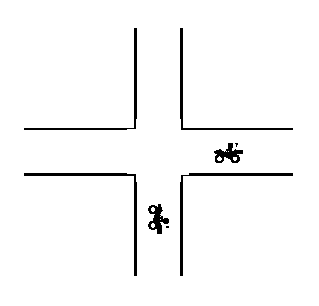
\includegraphics[scale=1.5]{crossroads.eps}
\caption{Who goes first?}
\label{ch6:fig:crossroads}
\end{figure}
The drivers can either wait (w) and stop at the crossroad, or go on (g).
We will represent this as a 2 player game, with the following strategic form
\begin{center}
\begin{tabular}{c | c  c}
& g & w\\
\hline
G & -10, -10 & 2, 0  \\
W & 0, 2 & -1, -1
\end{tabular}
.
\end{center}

There are four outcomes for this game: players can have an accident (which matches the choice of strategies ([G],[g])), or Player 1 waits ([W],[g]), or Player 2 waits ([G],[w]), or both wait ([W],[w]). \\
The game has 3 Nash Equlibria: $([G],[w])$, $([W],[g])$, and $(\frac{3}{13}[G] + \frac{10}{13}[W], \frac{3}{13}[g] + \frac{10}{13}[w])$. We know that, since the players are rational, they are \emph{going to play at a Nash equilibrium}. \\
What does this mean? It means that for this games, Player 1 may pick [G], [W] or 0.5[G] + 0.5[W] depending on what he \emph{believes} Player 2 is going to do. The same occurs for Player 2.
However, it may very well be the case that Player 1 thinks Player 2 is going to stop, and the reverse holds for Player 2. As a consequence, the players may crash rationally even if neither one played the randomized equilibrium.

Of course, in practice, we know several ways to solve the crossroad problem. In Belgium, the \emph{law} states that we should always let the one arriving from the right go first. If we break the law, we face dire consequences (first, we may have an accident, and second, if we get caught, we can be heavily reprimanded).

Another way to solve this problem is by installing a \emph{traffic light} at the crossroad. At every instant, the red light actually suggests to the players an outcome for the game ([G],[w]) or ([W],[g]). Most of the time, players follow this recommendation since if we receive a signal not to go, we know the other one is signalled to go. Thus, if we do not follow recommendations, we actually chose to have an accident.

Yet another way to solve this problem would be through communication. We could imagine a situation where the players are able to send signals to each others, and decide (perhaps by tossing a coin) on a suitable outcome for the game. A reasonable strategy for the players would be to pick the outcome ([G],[w]) or ([W],[g]), each with probability $1/2$.

\label{ch5:example:crossroads1}
\end{example}

In the following, we will be considering games in strategic form $\Gamma = (N,C,u)$.
Recall that in this case, the \emph{outcomes of the games} are associated with pure strategies (hence, we can refer to $C$ as the set of outcomes).
Our players will try to find an agreement about which outcome should occur. As presented in the example, they may agree to randomize on these outcomes.

\begin{definition}[Correlated strategy]
Given a game in strategic form $\Gamma = (N,C,u)$, the set of \emph{correlated strategies} is
$$ \Delta(C) = \Delta(\times_{i \in N} C_i). $$
\end{definition}

As always, our players' decision will be driven by their utility functions.
\begin{definition}[Expected payoff for correlated strategy]
Given a game $\Gamma = (N, C, (u_i)_{i \in N})$  the payoff of player $i \in N$ for a correlated strategy $\mu \in \Delta(C)$
$$U_i(\mu) = \sum_{c \in C} \mu(c) \cdot u_i(c).$$
\end{definition}

Before moving further, let us give more explanations about \emph{why} do we call these $\mu$ \emph{correlated strategies}?
Any given a randomized strategy profile $\sigma \in \times_{i \in N} \Delta(C_i)$ corresponds to a unique correlated strategy $\mu$, where
$$\forall c = (c_i)_{i \in N} \in C, \mu(c) = \prod_{i \in N} \sigma_i(c_i). $$
However, the reverse does not hold: when choosing their strategies \emph{independently} of one another,  there are some correlated strategy that cannot be reached by the players (this is shown in the next example). Thus the name: in correlated equilibria, the probability distribution of the actions of the different players are allowed to be correlated with each other, which enables much more possibilities than in classical standard games.

\begin{example}
Assume, in the crossroads example, that the player want to implement the \emph{correlated strategy} $0.5([G], [w]) + 0.5 ([W], [g])$. To do so, Player 1 can for example toss a coin, and communicate the result to Player 2 (assuming Player 1 is truthful).  Alternatively, they can make use of a red-light (if present).\\
Something they can not do, however, is to play according to a randomized strategy - say $\alpha_1[G] + (1-\alpha_1)[W]$ for the first player, and $\alpha_2[g] + (1-\alpha_2)[w]$ for the second.
Indeed, this requires
$$ \mu([G], [g]) = \alpha_1 \alpha_2 = 0; \mu([G], [w]) = \alpha_1 (1-\alpha_2) = 0.5, \mu([W], [g]) = (1-\alpha_1) (\alpha_2) = 0.5, $$
which is impossible.
\end{example}
We can already conclude that considering correlated strategies opens new horizons to the players, because this allows for outcomes that are impossible to reach when players chose their moves independently of each other.\\

Naturally, one may ask the question ``how are the players able to implement a correlated strategy''?
This is where the mediator comes in to play. It has a role similar to that of the traffic light in Example \ref{ch5:example:crossroads1}.
The role of a mediator is to:
\begin{enumerate}
\item{Describe a correlated strategy to the players. }
\item{Privately sample an outcome of the game following the correlated strategy. }
\item{Secretely inform each player of their own strategies (but not of that of the others).}
\end{enumerate}








\section{Correlated equilibria}

We now investigate the notion of \emph{correlated equilibria}.
To give a intuitive meaning to the concept and its shadow zones, we consider that the ultimate choice made by a player is up to that player.
As seen in Figure \ref{figureDrawnByMatt}, this implies that we need to study an augmented game where, on top of their own moves, player have the possibility to follow or not the recommendations of the mediator.

\begin{figure}[!ht]
\centering
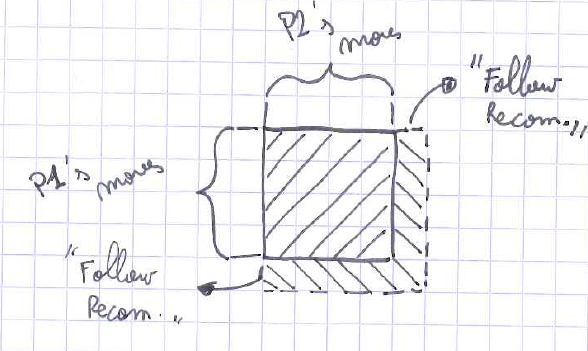
\includegraphics[scale=0.5]{drawingMatt.PNG}
\caption{Players must chose rationally if they follow the recommendations of the mediator.}
\label{figureDrawnByMatt}
\end{figure}

A correlated equilibrium occurs when it is a Nash equilibrium for players to follow the recommendations.
It is therefore natural to study what happens when one wishes to not follow recommendations. In this context, we first study the concept of binding contract.

\subsection{Binding contracts}
\label{ch5:sec:cont}

In this context, we assume that the players have the options to sign a binding contract with the mediator. The recommendations of the mediator will vary according to which players signed the contract.
The goal of the mediator is to make the contract attractive to everybody.


\begin{definition}[Contract]
Given a game $\Gamma = (N,C,u)$, a contract $\tau$ is a function
$$ \tau : S \subseteq N \rightarrow \Delta \times_{i \in S}(C_i), $$
that assigns to each subset of players $S$ the correlated strategy  they will play if $S$ signs the contract and $N \backslash S$ does not.
\end{definition}

In the definition above, $\tau(N)$ is a correlated strategy as defined in the previous section. For any other $S \subset N$, $\tau(S)$ is also a correlated strategy, but which is going to be implemented only by the members of the set $S$ that sign the contract.
The players who do not sign the contract are free to choose an action in their action set.

The following follows directly from the definition of Nash Equilibrium.
\begin{proposition}[Correlated equilibrium with binding contract]
Consider a game $\Gamma = (N,C,u)$, and a contract $\tau$ for this game. The correlated strategy $\tau(N)$ is a correlated equilibrium if and only if
$$ \max_{c_i \in C_i} \sum_{c_{-i} \in C_{-i}} \tau(N \backslash i, c_{-i})u_i(c_i, c_{-i}) \leq \sum_{c \in C} \tau(N, c) u_{i}(c),$$
where for $S \subseteq N$, $c \in \times_{i \in S} C_i$, $\tau(S,c)$ is the probability that the players in $S$ having signed the contract play the strategy $c$.
\end{proposition}
The above simply states that one won't sign a contract if doing so allows him to obtain an higher payoff.

Assume now that, as a mediator, you wish to propose a contract where $\tau(N)$ is a correlated equilibrium. A player won't sign the contract unless he has some incentive to do so. One way to do so is by using a threat, by choosing  a $\tau(N \backslash i)$ that would guarantee that $i$ would prefer to sign. In order to do this, we may use its \emph{minimax value}.

\begin{definition}[Minimax]
The \emph{minimax value} for player $i$ is defined as
\begin{align*}
v_i = \min_{\tau_{-i} \in \Delta(C_{-i})} \max_{c_i \in C_i} \sum_{c_{-i} \in C_{-i}} \tau_{-i}(c_{-i}) \cdot u_i(c_{-i}, c_i).
\end{align*}
\end{definition}
\begin{example}
\label{ch5:ex:minimax}
Alice and Bob plan to meet in the evening. There are two options available: either to go to the cinema, or to the ballet.
Alice prefers to go to the ballet, and Bob to the cinema. They find it hard to decide and decide to ask Charles to mediate their dispute by providing them with a binding contract and a correlated equilibrium.

Their payoffs and moves are summarized in the table below (Alice is Player 1, Bob is Player 2).
\begin{center}
\begin{tabular}{c | c  c}
& c & b\\
\hline
C & 2, 3 & -1, -1  \\
B & 1, 1 & 3, 2
\end{tabular}
.
\end{center}

We begin by computing the minimax value $v_1$. Assume that Bob plays $c$ with probability $\beta$, and $b$ with probability $1-\beta$.
The payoff of Alice are given by
$$ u_{1}(C, \beta[c] + 1-\beta[b]) = 3\beta - 1, u_{1}(B, \beta[c] + 1-\beta[b]) = -2\beta + 3.  $$
The minimax strategy for Bob is to pick $\beta = 4/5$, and the minimax value for Alice is $v_1 = 7/5$.

For $v_2$, we apply the same technique: if Alice plays $C$ with probability $\alpha$, we have
$$ u_{2}(\alpha [C] + (1-\alpha)[B], c) = 2 \alpha - 1, u_{2}(\alpha [C] + (1-\alpha)[B], b) = -3\alpha + 2.  $$
The minimax strategy for Alice is to pick $\alpha = 1/5$, and the minimax value for Bob is $v_2 = 7/5$.

In conclusion, Alice and Bob will sign any contract proposed by Charles as long as their expected payoff is at least $7/5$. In particular, Charles could tell them to both go to the cinema, or to both go to the ballet.
We  discuss in Chapter \ref{chap:Bar} tools allowing Charles to select an appropriate correlated strategies among those agreeable to Alice and Bob (see Example \ref{example:AliceBobCinemaBargain}).

\end{example}

The next result allow us the characterize all the correlated strategies for which there is a contract making them a correlated equilibria.
\begin{theorem}
Consider a correlated strategy $\mu$. There exists a contract $\tau$ with $\tau(N) = \mu$ in which all players signing is an equilibrium if and only if $U_i(\mu) \geq v_i$ for all $i \in N$, where $v_i$ is the minimax value for player $i$.
\label{thm:minimaxcor}
\end{theorem}

\vspace{1cm}


\subsection{Correlated equilibria for games in strategic form}
\label{ch5:sec:cor}



Let us assume now that the players do not have to sign any contract, so they are free to follow the plan of the mediator or to deviate from it during the game. To ensure that the latter case does not occur, a correlated equilibrium for such a game in \emph{strategic form} must satisfy the following strategic incentive constraints:
\begin{definition}[Strategic incentive constraints]
A correlated strategy $\mu$ satisfies to the \emph{strategic incentive constraints} if
\begin{align*}
	U_i(\mu) \geq \sum_{c \in C} \mu(c) \, u_i(c_{-i}, \; \delta(c_i)), \quad \forall i \in N, \ \forall \delta : C_i \rightarrow C_i,
\end{align*}
where $c = (c_{-i}, c_i)$, $c_{-i}$ being the strategy of the players other than $i$, and where $\delta(c_i)$ is a cheating function that replaces any strategy $c_i \in C_i$ suggested by the mediator by a strategy $\delta(c_i) \in C_i$. \\
A correlated strategy satisfying the strategic incentive constraints is said to be \emph{incentive compatible.}
\label{ch6:def:incentive}
\end{definition}


These constraints require that the players cannot improve their payoff by deviating from the correlated strategy $\mu$ suggested by the mediator. Note that cheating would be perfectly rational if it was the case.
Indeed, when a mediator dictates to a player what he should do to follow the correlated strategy, the player may infer a probability distribution on the other players moves.
More precisely, if a mediator implementing $\mu$ tells $i$ to play $c_i$, then the other players are going to play according to
$$ \sigma_{-i}(c_{-i}) = \frac{\mu(c_{i}, c_{-i})}{ \sum_{e_{-i} \in C_{-i}} \mu_(c_i, e_{-i})}.$$
Given this knowledge, a rational player would naturally compute his best response to $\sigma_{-i}(c_{-i})$ and, if this brings him a better payoff than the one obtained by following the recommendation, he will adopt the best response.

\begin{example}
For the crossroads example, the correlated strategy $\mu = 0.5([G], [w]) + 0.5 ([W],[g])$ is incentive compatible.
Indeed, if a player is told to slow down, this player can infer that the other player has been told to keep going. Thus, if the first player decided to cheat and kept moving, an accident would surely happen.\\
On the other hand, the correlated strategy $\mu = ([W],[w])$ cannot be incentive compatible. Indeed, since the other player is being told to slow down, the best response is just to keep moving.
\end{example}

 Note that, because of the cheating function, the  formulation of Definition \ref{ch6:def:incentive} describes a polytope with an exponential number of inequalities. To avoid this problem, we can equivalently rewrite the conditions with a polynomial number of inequalities as follows:
\begin{align*}
	\sum_{c_{-i} \in C_{-i}} \mu(c) \, \big( u_i(c_{-i}, \; c_i) - u_i(c_{-i}, \; e_i) \big) \geq 0, \quad \forall i \in N, \ \forall c_i \in C_i, \ \forall e_i \in C_i.
\end{align*}

Finally, note that we may have several possible incentive compatible correlated strategies. The mediator still needs to pick one.
One way to do this is by maximizing some objective function. For example,
one may try to maximize $U_1(\mu) + U_2(\mu)$ (total amount of utility). The good news is that such objective functions are \emph{linear} in the variables $\mu(c)$, $c \in C$, and thus for instance, \emph{the problem of finding an incentive compatible mechanism that maximizes total payoff is a linear program}.

\section{Correlated equilibria for Bayesian games}
\label{ch5:sec:bay}




People are able to cheat when it is in their interest, but what about lying? In the context of Bayesian games (see Section \ref{ch2:bayesianGames}), players now have access to private information
able to shape the game. In order to make sound recommendations, the mediator needs access to this information. But maybe giving a false statement may steer the recommendations in your favor...

We now consider \emph{Bayesian games with communication}. Recall that a Bayesian game is defined as $\Gamma = (N,C,T,p,u)$, where the $T = (T_i)_{i \in N}$ are the \emph{types} of each players,
$p = (p_{i})_{i \in N}$ where $p_i : T_i \rightarrow \Delta(T_{-i})$ and the payoffs are defined as $u = (u_i)_{i \in N}$ with
$$u _i : T \times C \rightarrow \reels. $$
That is, the payoffs of the players now depend on their types!

The mediator now needs to prepare recommendations for any combination of player times.
\begin{definition}[(Bayesian) correlated strategy]
Given a bayesian game $\Gamma = (N,C,T,p,u)$, a Bayesian correlated strategy is a function of the form
$$ \mu : T \rightarrow \Delta(C).$$
For a correlated strategy $\mu$, the payoff of player $i$ given his type $t_i$, is given by:
\begin{align*}
	U_i(\mu \; | \; t_i) = \sum_{t_{-i} \in T_{-i}} \sum_{c \in C} p_i(t_{-i} \; | \; t_i) \, \mu(c \; | \; t) \, u_i(c, \; t),
\end{align*}
where $t = (t_{-i}, t_i)$ and $T_{-i}$ are the set of possible combinations of types for the  players other than $i$.
\end{definition}

The task of a mediator can now be described as
\begin{enumerate}
\item Propose to the players a set of correlated strategies $\mu(\cdot | t)$, one per combination of types $t \in T$.
\item Collect the types of the players.
\item Privately compute the outcome of the correlated strategy.
\item Secretly communicate his recommendations to each players.
\end{enumerate}






The problem is that,  to guarantee a desired outcome, the mediator needs not only propose an incentive compatible strategy for each combination  of types, be he must also be sure that he knows the correct types for the players for doing the recommendations.

\begin{example}
Back at our crossroads!
Consider the following situation. You are an engineer working on a \emph{``smart crossroad''} project.
The idea is the following: some drivers (type V for VIP) are more important than others (type R for Regular). For example, those driving an ambulance should have priority on those who are just doing their groceries.\\
The cars of your city have been equipped with rudimentary devices, that broadcast whether they are VIP drivers or not. We would like to allow the VIP to pass whenever they are in the presence of regular drivers. \\
Assume the following bayesian model for the game:
\begin{center}
\begin{tabular}{c | c  c}
R vs R & g & w\\
\hline
G & -10 / -10 & 2 / 0  \\
W & 0 / 2 & -1 / -1
\end{tabular}
\begin{tabular}{c | c  c}
R vs V & g & w\\
\hline
G & -30 / -10 & 2 / -1  \\
W & 1 / 5 & -1 / -5
\end{tabular}
\begin{tabular}{c | c  c}
V vs R & g & w\\
\hline
G & -10 / -30 & 5 / 1  \\
W & -1 / 2 & -5 / -1
\end{tabular}
\begin{tabular}{c | c  c}
V vs V & g & w\\
\hline
G & -10 / -10 & 2 / 0  \\
W & 0 / 2 & -1 / -1
\end{tabular}
\end{center}
Regarding the beliefs functions $p$, we may assume $p(V | R) = p(V | V) =  p(V) = 0.1$, $p(R | R) = p(R | V) = p(R) = 0.9$ as objective probabilities.

The problem is that most resident of the city are talented engineers, and they can hack the broadcast device with ease.
Could you build a policy, using red-lights, that allows VIP drivers to have priority over regular ones, but that would also discourage all drivers to hack their devices?



A naive approach would be to consider each of the four cases separately, and prepare one incentive compatible mechanism for each which, for example, would maximize total payoff.
In our case, this yields
\begin{itemize}
\item $\mu(\cdot | RR) = 0.5([G], [w]) + 0.5([W], [g])$,
\item $\mu(\cdot | RV) = ([W], [g])$,
\item $\mu(\cdot | VR) = ([G], [w])$,
\item $\mu(\cdot | VV) = 0.5([G], [w]) + 0.5([W], [g])$,
\end{itemize}

Assume now that, as a regular driver, you were aware that the above was the strategy implemented at the crossroads. Would you hack your broadcast device to appear as a VIP?

Assume you broadcast as a regular driver. Your payoff is then going to be
$$ U_1(\mu | R) =  p(R) u_1(\mu(\cdot | RR) | RR) + p(V)  u_1(\mu(\cdot | RV) | RV) = 0.9 \cdot 1 + 0.1 \cdot 1 = 1. $$
Indeed, with probability $p(R)$, the other player is of type $R$, so the recommendations are then given by $\mu(\cdot | RR)$. With probability $p(V)$, the other player is of type $V$, so we receive recommendations according to $\mu(\cdot | RV)$.
If, instead we decided to broadcast your type as VIP, your payoff would become
$$ p(R) u_1(\mu(\cdot | VR) | RR) + p(V)  u_1(\mu(\cdot | VV) | RV) = 0.9 \cdot 2 + 0.1 \cdot 1.5 = 2.85. $$
It is important to understand that we would receive the payoffs of a regular player, but the recommendations of a VIP driver. Thus, we get priority over regular drivers, and equal chances to go or wait versus a VIP driver.


In conclusion, yes, it would be rational to hack the device. The design of the proposed strategy did not take this into account.
\end{example}


\begin{definition}[Incentive Compatibility]
A bayesian correlated strategy $\mu : T \rightarrow \Delta C$ is incentive compatible if it satisfies to the constraints
\begin{align*}
	U_i(\mu \; | \; t_i) \geq U_i^*(\mu, \; \delta_i, \; s_i \; | \; t_i), \quad \forall i \in N, \ \forall t_i \in T_i, \ \forall s_i \in T_i, \ \forall \delta_i : C_i \rightarrow C_i,
\end{align*}
with
\begin{align*}
	U_i^*(\mu, \; \delta_i, \; s_i \; | \; t_i) = \sum_{t_{-i} \in T_{-i}} \sum_{c \in C} p_i(t_{-i} \; | \; t_i) \, \mu(c \; | \; t_{-i}, s_i) \, u_i\big( \; (c_{-i}, \; \delta_i(c_i)) \;, \; t \big),
\end{align*}
where $t_i$ is the type of $i$, $s_i$ is the type that $i$ reveals to the mediator and $\delta_i$ is the function chosen by player $i$ that, for any action $c_i$ that can be suggested by the mediator, chooses an action $\delta_i(c_i)$ to play instead.
\label{incentiveCompatible}
\end{definition}

These constraints impose that the players neither have interest to lie on their type, nor to deviate from the correlated strategy $\mu$ suggested by the mediator.


\begin{example}


We now conclude our crossroad example by presenting a mechanism satisfying to the incentive constraints for the bayesian game.

One may verify that the following strategy is incentive compatible
\begin{itemize}
\item $\mu(\cdot | RR) = 0.5([G], [w]) + 0.5([W], [g])$,
\item $\mu(\cdot | RV) = ([W], [g])$,
\item $\mu(\cdot | VR) = ([G], [w])$,
\item $\mu(\cdot | VV) = 1/3([G],[g]) + 1/3([G], [w]) + 1/3([W], [g])$.
\end{itemize}


The approach is quite dangerous: in order to deter a regular player from lying, we tell him that VIPs tend to crash into VIPs. Since crashing into a VIP has a very high cost for a regular driver, he then has no interest into lying.
\label{chap8cleverstuff}
\end{example}



\subsection{Collective choice problems}
\label{ch5:subs:coll}
In this section, we mention a special type of Bayesian games with communications, known as \emph{Collective choices problems}.\\
These problems refer to situations where we seek to make a decision based on the type of players in a population.
A typical example of this are \emph{voting problems}, where each citizen's type corresponds to preferences in candidates, and the goal
is to chose which candidate to elect (see e.g. \cite[Chapter 9]{ShLeMSAG}). In this case, we which to establish rules under which it is in each citizen's interest to
report his preferences truthfully.

With this in mind, we assume that a mediator is going to gather the types of the players and decide on the outcome of a game.
In order for the player to be incentivized to divulge their true types, the mediator must pick an incentive compatible strategy in the following sense:
\begin{definition}[(Collective choice) incentive compatibility]
For a collective choice problem, a Bayesian correlated strategy $\mu : T \rightarrow \Delta C$ is incentive compatible if it satisfies to the constraints
\begin{align*}
	U_i(\mu \; | \; t_i) \geq U_i^*(\mu,  \; s_i \; | \; t_i), \quad \forall i \in N, \ \forall t_i \in T_i, \ \forall s_i \in T_i,
\end{align*}
with
\begin{align*}
	U_i^*(\mu, \;  s_i \; | \; t_i) = \sum_{t_{-i} \in T_{-i}} \sum_{c \in C} p_i(t_{-i} \; | \; t_i) \, \mu(c \; | \; t_{-i}, s_i) \, u_i\big( \; (c_{-i}, \; c_i )\;, \; t \big),
\end{align*}
where $t_i$ is the type of $i$, $s_i$ is the type that $i$ reveals to the mediator.
\end{definition}
%\begin{example}
%Elections time are near, and three candidates are available: $a$, $b$ and $c$.
%The population expresses preferences of the sort $a \succ b \succ c$. For such an agent, if his first choice gets elected, this amounts to a utility payoff of 2, the second choice to a payoff of 1, and the last choice to a payoff of -2 (turns out data show people tend to really dislike their last choice).
%
%For the election process, we wish to maximize the utility gained by the voters. Assume three sorts of voters are present, with preferences
%$$
%\begin{aligned}
%& t_1 = \{a \succ b \succ c\},\\
%& t_2 = \{b \succ c \succ a\},\\
%& t_3 = \{c \succ a \succ b\}.\\
%\end{aligned}
%$$
%
%
%The election is based on \emph{Condorcet conditions}: for each candidate, we count the number of times that candidate is preferred to another one. For example, if somehow states that $a \succ b \succ c$, then $a$ is preferred twice (once over $b$, and once over $c$). The candidate who is the most preferred is then elected.
%
%Assume there are 100 participants, where we can find three preferences:
%
%
%
%\end{example}
%


\section{Moral hazards and adverse selection}

The problem faced by mediators having to give incentive for player to be truthful about their types and to follow recommendations is ubiquitous in the insurance industry. The following definition is extracted from \cite[p. 263]{MyGTAO}.
\begin{definition}[{Moral hazard and adverse selection }]
\emph{Moral hazard} is the need to give players an incentive to implement recommended actions.
\emph{Adverse selection} is the need to give players an incentive to report information honestly.
\end{definition}

  Overall, the contents of this chapter can be split into four categories:

  \begin{tabular}{c | c | c}
  & With moral hazard & Without moral hazard \\
  \hline
  With adverse selection   & Section \ref{ch5:sec:bay} &  Subsection \ref{ch5:subs:coll} \\
  \hline
  Without adverse selection  & Subsection \ref{ch5:sec:cor}  & Subsection \ref{ch5:sec:cont} \\
  \end{tabular}








\ifx \globalmark \undefined %% This is default.
\bibliographystyle{apalike}
\bibliography{../gametheorybibliography}
	\end{document}
\else

\fi
